% Options for packages loaded elsewhere
\PassOptionsToPackage{unicode}{hyperref}
\PassOptionsToPackage{hyphens}{url}
%
\documentclass[
]{article}
\usepackage{amsmath,amssymb}
\usepackage{lmodern}
\usepackage{ifxetex,ifluatex}
\ifnum 0\ifxetex 1\fi\ifluatex 1\fi=0 % if pdftex
  \usepackage[T1]{fontenc}
  \usepackage[utf8]{inputenc}
  \usepackage{textcomp} % provide euro and other symbols
\else % if luatex or xetex
  \usepackage{unicode-math}
  \defaultfontfeatures{Scale=MatchLowercase}
  \defaultfontfeatures[\rmfamily]{Ligatures=TeX,Scale=1}
\fi
% Use upquote if available, for straight quotes in verbatim environments
\IfFileExists{upquote.sty}{\usepackage{upquote}}{}
\IfFileExists{microtype.sty}{% use microtype if available
  \usepackage[]{microtype}
  \UseMicrotypeSet[protrusion]{basicmath} % disable protrusion for tt fonts
}{}
\makeatletter
\@ifundefined{KOMAClassName}{% if non-KOMA class
  \IfFileExists{parskip.sty}{%
    \usepackage{parskip}
  }{% else
    \setlength{\parindent}{0pt}
    \setlength{\parskip}{6pt plus 2pt minus 1pt}}
}{% if KOMA class
  \KOMAoptions{parskip=half}}
\makeatother
\usepackage{xcolor}
\IfFileExists{xurl.sty}{\usepackage{xurl}}{} % add URL line breaks if available
\IfFileExists{bookmark.sty}{\usepackage{bookmark}}{\usepackage{hyperref}}
\hypersetup{
  hidelinks,
  pdfcreator={LaTeX via pandoc}}
\urlstyle{same} % disable monospaced font for URLs
\usepackage[margin=1in]{geometry}
\usepackage{longtable,booktabs,array}
\usepackage{calc} % for calculating minipage widths
% Correct order of tables after \paragraph or \subparagraph
\usepackage{etoolbox}
\makeatletter
\patchcmd\longtable{\par}{\if@noskipsec\mbox{}\fi\par}{}{}
\makeatother
% Allow footnotes in longtable head/foot
\IfFileExists{footnotehyper.sty}{\usepackage{footnotehyper}}{\usepackage{footnote}}
\makesavenoteenv{longtable}
\usepackage{graphicx}
\makeatletter
\def\maxwidth{\ifdim\Gin@nat@width>\linewidth\linewidth\else\Gin@nat@width\fi}
\def\maxheight{\ifdim\Gin@nat@height>\textheight\textheight\else\Gin@nat@height\fi}
\makeatother
% Scale images if necessary, so that they will not overflow the page
% margins by default, and it is still possible to overwrite the defaults
% using explicit options in \includegraphics[width, height, ...]{}
\setkeys{Gin}{width=\maxwidth,height=\maxheight,keepaspectratio}
% Set default figure placement to htbp
\makeatletter
\def\fps@figure{htbp}
\makeatother
\setlength{\emergencystretch}{3em} % prevent overfull lines
\providecommand{\tightlist}{%
  \setlength{\itemsep}{0pt}\setlength{\parskip}{0pt}}
\setcounter{secnumdepth}{5}
\usepackage{booktabs}
\usepackage{color}
%\usepackage{amsmath}
\usepackage{amssymb}
\usepackage{amsfonts}

\usepackage{framed}
\setlength{\fboxsep}{.8em}
%
% \newenvironment{blackbox}{
%   \definecolor{shadecolor}{rgb}{0, 0, 0}  % black
%   \color{white}
%   \begin{shaded}}
%  {\end{shaded}}
%
% \usepackage{tcolorbox}
%
% \newtcolorbox{blackbox}{
%   colback=black,
%   colframe=orange,
%   coltext=white,
%   boxsep=5pt,
%   arc=4pt}
\ifluatex
  \usepackage{selnolig}  % disable illegal ligatures
\fi
\usepackage[]{natbib}
\bibliographystyle{plainnat}

\author{}
\date{\vspace{-2.5em}}

\begin{document}

{
\setcounter{tocdepth}{2}
\tableofcontents
}
\hypertarget{ptapp}{%
\section{Process Tracing Application: Inequality and Democracy}\label{ptapp}}

In this chapter, we demonstrate how causal-model-based process-tracing works using real data. We undertake this illustration on a substantive issue that has been of central interest to students of comparative politics for decades: the causes of democratization. As the literature and range of arguments about democratization are vast, we focus on just a piece of the debate---specifically on causal claims about the relationship between economic inequality and democratization, with particular attention to the work of \citet{boix2003democracy}, \citet{acemoglu2005economic}, and \citet{haggard2012inequality}. In this chapter, we demonstrate process tracing with causal models, while in a later chapter we demonstrate the integration of process-tracing with correlational analysis. Our focus in this chapter is on using process tracing to assess \emph{the case-level causal effect of inequality on democracy.}

\hypertarget{inequality-and-democratization-the-debate}{%
\subsection{Inequality and Democratization: The Debate}\label{inequality-and-democratization-the-debate}}

Sociologists, economists, and political scientists have long theorized and empirically examined the relationship between inequality and democracy (e.g., \citet{dahl1973polyarchy}, \citet{bollen1985political}, \citet{acemoglu2005economic}, \citet{boix2003democracy}, \citet{ansell2014inequality}). In recent years, the work of \citet{boix2003democracy}, \citet{acemoglu2005economic}, and \citet{ansell2014inequality} represent major theoretical advances in specifying when and how inequality might generate transitions to democracy (as well as its persistence, which we bracket here). The first and third of these books also provide large-n cross-national and historical tests of their theories' key correlational predictions. \citet{haggard2012inequality}, moreover, derive causal process observations from a large number of ``Third Wave'' cases of democratization in order to examine these theories' claims about the centrality of distributional issues to regime change. We provide a very condensed summary of the core logic of \citet{boix2003democracy} and \citet{acemoglu2005economic} before seeking to translate that logic into a causal model for the purposes of process tracing, using a transformed version of Haggard and Kaufman's causal-process data.

We briefly summarize the core logics of and differences among these three sets of arguments here, bracketing many of their moving parts to focus on the basic theorized relationship between inequality and democracy. Both Boix's and Acemoglu and Robinson's theories operate within a Meltzer-Richard (\citet{meltzer1981rational}) framework in which, in a democracy, the median voter sets the level of taxation-and-transfer and, since mean income is higher than median income, benefit from and vote for a positive tax rate, implying redistribution from rich to poor. The poorer the median voter, the more redistribution she will prefer. Democracy, with its poorer median voter, thus implies greater redistribution than (rightwing) authoritarianism---a better material position from the poor at the expense of the rich elite. Thus, in each of these approaches, struggles over political regimes are conflicts over the distribution of material resources.

In Boix's model, the poor generally prefer democracy for its material benefits. When they mobilize to demand regime change, the rich face a choice as to whether to repress or concede, and they are more likely to repress as inequality is higher since, all else equal, they have more to lose from democracy. Thus, with the poor always preferring democracy over rightwing authoritarianism, inequality reduces the prospects for democratization.

In Acemoglu and Robinson's model, inequality simultaneously affects the expected net gains to democracy for both rich and poor. At low levels of inequality, democracy is relatively unthreatening to the elite, as in Boix, but likewise of little benefit to the poor. Since regime change is costly, the poor do not mobilize for democracy when inequality is low, and democratization does not occur. At high levels of inequality, democracy is of great benefit to the poor but has high expected costs for the elite; thus, democratization does not occur because the elite repress popular demands for regime change. In Acemoglu and Robinson's model, democracy emerges only when inequality is at middling levels: high enough for the poor to demand it and low enough for the rich to be willing to concede it.

Ansell and Samuels, finally, extend the distributive politics of regime change in two key ways. First, they allow for a two-sector economy, with a governing elite comprising the landed aristocracy and an urban industrial elite excluded from political power under authoritarian institutions. Total inequality in the economy is a function of inequality in the landed sector, inequality in the industrial sector, and the relative size of each. Second, authoritarian (landed) elites can tax the industrial bourgeoisie, thus giving the industrial elite an incentive to seek constraints on autocratic rule. Third, in Ansell and Samuels' model, rising industrial inequality means a rising industrial elite, generating a larger gap between them and industrial workers, though the industrial masses are richer than the peasantry. A number of results follow, of which we highlight just a couple. Rising land inequality reduces the likelihood of bourgeois rebellion by giving the landed elite greater repressive capacities and increasing their expected losses under democracy. As industrial inequality rises, however, the industrial elite have more to lose to confiscatory taxation and thus greater incentive to push for partial democracy (in which they have the ability to constrain the government, though the poor remain politically excluded) as well as greater resources with which to mobilize and achieve it. Full democracy, brought on by joint mass and bourgeois rebellion, is most likely as the industrial sector grows in relative size, giving the urban masses more to lose to autocratic expropriation and more resources with which to mobilize and rebel.

These three theoretical frameworks thus posit rather differing relationships between inequality and democracy. Taking these theoretical logics as forms of background knowledge, we would consider it possible that inequality reduces the likelihood of democracy or that it increases the likelihood of democracy. Yet one feature that all three theories have in common is a claim that distributional grievances drive demands for regime change. Moreover, in both Boix and Acemoglu and Robinson, less economically advantaged groups are, all else equal, more likely to demand democracy the worse their relative economic position. Ansell and Samuels' model, on the other hand, suggests that relative deprivation may cut both ways: while poorer groups may have more to gain from redistribution under democracy, better-off groups have more to fear from confiscatory taxation under autocracy. In all three frameworks, \emph{mobilization} by groups with material grievances is critical to transitions to democracy: elites do not voluntarily cede power.

In their qualitative analysis of ``Third Wave'' democratizations, Haggard and Kaufman point to additional factors, aside from inequality, that may generate transitions. Drawing on previous work on 20th century democratic transitions (e.g., \citet{huntington1993third}, \citet{linz1996problems}), they pay particular attention to international pressures to democratize and to elite defections.

\hypertarget{a-structural-causal-model}{%
\subsection{A Structural Causal Model}\label{a-structural-causal-model}}

We now need to express this background knowledge in the form of a structural causal model. Suppose that we are interested in the case-level causal effect of inequality on democratization of a previously autocratic political system. Suppose further, to simplify the illustration, that we conceptualize both variables in binary terms: inequality is either high or low, and democratization either occurs or does not occur. This means that we want to know, for a given case of interest, whether high inequality (as opposed to low inequality) causes democracy to emerge, prevents democracy from emerging, or has no effect (i.e., with democratization either occurring or not occurring independent of inequality). We can represent this query in the simple, high-level causal model shown in Figure \ref{fig:dagdemochigh}. Here, the question, ``What is the causal effect of high inequality on democratization in this case?'' is equivalent to asking what the value of \(\theta^D\) is in the case, where the possible values are \(\theta_{00}^D, \theta_{01}^D, \theta_{10}^D\), and \(\theta_{11}^D\). We assume here that the case's nodal type, \(\theta^D\), is not itself observable, and thus we are in the position of having to make inferences about it.

Drawing on the grammar of causal graphs discussed in Chapter \ref{models}, we can already identify possibilities for learning about \(\theta^D\) from the other nodes represented in this high-level graph. Merely observing the level of inequality in a case will tell us nothing since \(I\) is not \(d-\)connected to \(\theta^D\) if we have observed nothing else. On the other hand, only observing the outcome---regime type---in a case \emph{can} give us information about \(\theta^D\) since \(D\) \emph{is} \(d-\)connected to \(\theta^D\). For instance, if we observe \(D=1\) (that a case democratized), then we can immediately rule out \(\theta_{00}^D\) as a value of \(\theta^D\) since this type does not permit democratization to occur. Further, conditional on observing \(D\), \(I\) is now \(d-\)connected to \(\theta^D\): in other words, having observed the outcome, we can additionally learn about the case's type from observing the status of the causal variable. For example, if \(D=1\), then observing \(I=1\) allows us additionally to rule out the value \(\theta_{10}^D\) (a negative causal effect).

Now, observing just \(I\) and \(D\) alone will always leave two nodal types in contention. For instance, seeing \(I=D=1\) (the case had high inequality and democratized) would leave us unsure whether high inequality caused the democratization in this case (\(\theta^D=\theta_{01}^D\)) or the democratization would have happened anyway (\(\theta^D=\theta_{11}^D\)). This is a limitation of \(X, Y\) data that we refer to in \citet{humphreys2015mixing} as the ``fundamental problem of type ambiguity.'' Note that this does not mean that we will be left indifferent between the two remaining types. Learning from \(X, Y\) data alone---narrowing the types down to two---can be quite significant, depending on our priors over the distribution of types. For example, if we previously believed that a \(\theta_{00}^D\) type (cases in which democracy will never occur, regardless of inequality) was much more likely than a \(\theta_{11}^D\) type (democracy will always occur, regardless of inequality) and that positive and negative effects of inequality were about equally likely, then ruling out the \(\theta_{00}^D\) and \(\theta_{10}^D\) values for a case will shift us toward the belief that inequality caused democratization in the case. This is because we are ruling out both a negative effect and the type of null effect that we had considered the most likely, leaving a null effect that we consider relatively unlikely.

\begin{figure}

{\centering 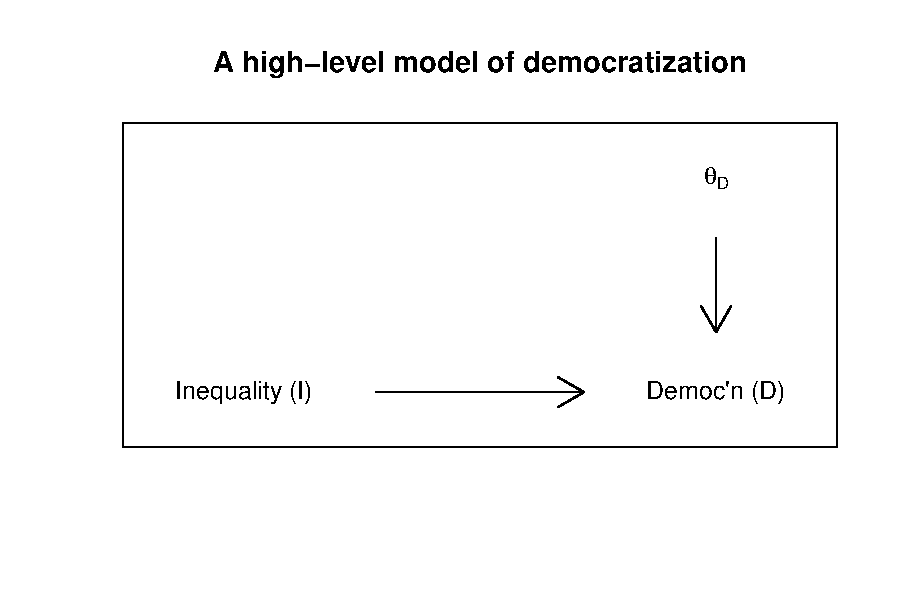
\includegraphics{ii_files/figure-latex/dagdemochigh-1} 

}

\caption{Simple democracy, inequality model}\label{fig:dagdemochigh}
\end{figure}

Nonetheless, we can increase the prospects for learning by \emph{theorizing} the relationship between inequality and democratization. Given causal logics and empirical findings in the existing literature, we can say more than is contained in Figure \ref{fig:dagdemochigh} about the possible structure of the causal linkages between inequality and democratization. And we can embed this prior knowledge of the possible causal relations in this domain in a lower-level model that is consistent with the high-level model that most simply represents our query.

If we were to seek to fully capture them, the models developed by Boix, Acemoglu and Robinson, and Ansell and Samuels would, each individually, suggest causal graphs with a large number of nodes and edges connecting them. Representing all variables and relationships jointly contained in these three models would take an extremely complex graph. Yet there is no need to go down to the lowest possible level---to generate the \emph{most} detailed graph---in order to increase our empirical leverage on the problem.

We represent in Figure \ref{fig:lowdem} one possible lower-level model consistent with our high-level model. Drawing on causal logics in the existing literature, we unpack the nodes in the high-level model in two ways:

\begin{enumerate}
\def\labelenumi{\arabic{enumi}.}
\item
  We interpose a mediator between inequality and democratization: mobilization (\(M\)) by economically disadvantaged groups expressing material grievances. \(M\) is a function of both \(I\) and of its own response-type variable, \(\theta^M\), which defines its response to \(I\). In inserting this mediator, we have extracted \(\theta^M\) from \(\theta^D\), pulling out that part of \(D\)'s response to \(I\) that depends on \(M\)'s response to \(I\).
\item
  We specify a second influence on democratization, international pressure (\(P\)). Like \(\theta^M\), \(P\) has also been extracted from \(\theta^D\); it represents that part of \(D\)'s response to \(I\) that is conditioned by international pressures.
\end{enumerate}

\begin{verbatim}
## Warning: Unknown or uninitialised column: `segment.alpha`.

## Warning: Unknown or uninitialised column: `segment.alpha`.

## Warning: Unknown or uninitialised column: `segment.alpha`.
\end{verbatim}

\begin{figure}

{\centering 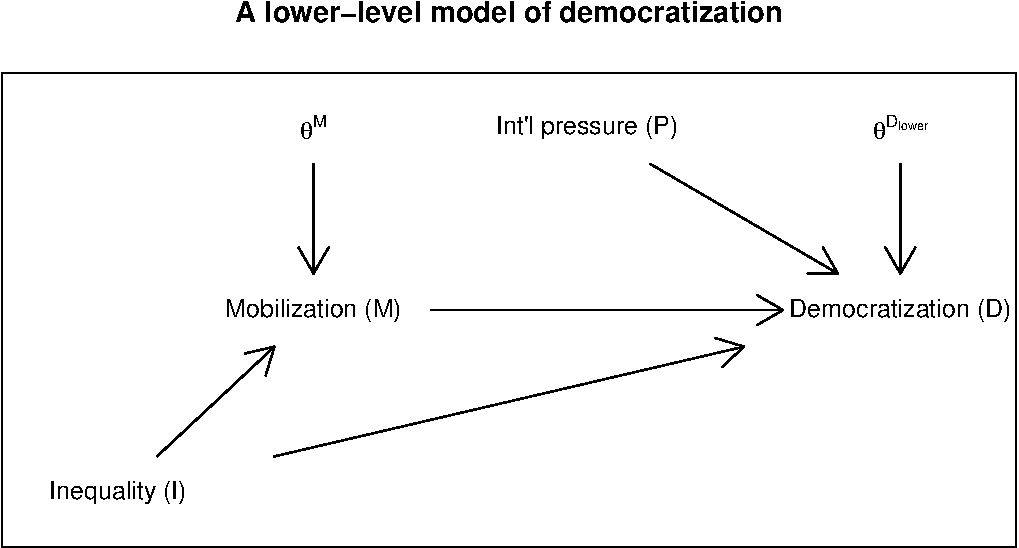
\includegraphics[width=.7\textwidth]{ii_files/figure-latex/lowdem-1} 

}

\caption{\label{fig:lowdem} A lower-level model of democratization in which inequality may affect regime type both directly and through mobilization of the lower classes, and international pressure may also affect regime type.}\label{fig:lowdem}
\end{figure}

In representing the causal dependencies in this graph, we allow for inequality to have (in the language of mediation analysis) both an ``indirect'' effect on democratization via mobilization and a ``direct'' effect. The arrow running directly from \(I\) to \(D\) allows for effects of inequality on democratization beyond any effects running via mobilization of the poor, including effects that might run in the opposite direction. (For instance, it is possible that inequality has a positive effect on democratization via mobilization but a negative effect via any number of processes that are not explicitly specified in the model.) The graph also implies that there is no confounding: since there is no arrow running from another variable in the graph to \(I\), \(I\) is modeled as exogenous.

The lower-level graph thus has two exogenous, response-type nodes that will be relevant to assessing causal effects: \(\theta^M\) and \(\theta^{D_{lower}}\). \(\theta^M\), capturing \(I\)'s effect on \(M\), ranges across the usual four values for a single-cause, binary setup: \(\theta_{00}^M, \theta_{01}^M, \theta_{10}^M\), and \(\theta_{11}^M\).

\(\theta^{D_{lower}}\) is considerably more complicated, however, because this node represents \(D\)'s response to three causal variables: \(I\), \(M\), and \(P\). One way to put this is that the values of \(\theta^{D_{lower}}\) indicate how inequality's direct effect will depend on mobilization (and vice-versa), conditional on whether or not there is international pressure. We need more complex notation than that introduced in Chapter 5 in order to represent the possible response types here.

The result is \(2^8=256\) possible response types for \(D\). With 4 response types for \(M\), we thus have 1024 possible combinations of causal effects between named variables in the lower-level graph. How do these lower-level response types map onto the higher-level response types that are of interest? In other words, which combinations of lower-level types represent a positive, negative, or zero causal effect of inequality on democratization?

To define a causal effect of \(I\) in this setup, we need to define the ``joint effect'' of two variables as being the effect of changing both variables simultaneously (in the same direction, unless otherwise specified). Thus, the joint effect of \(I\) and \(M\) on \(D\) is positive if changing both \(I\) and \(M\) from \(0\) to \(1\) changes \(D\) from \(0\) to \(1\). We can likewise refer to the joint effect of an increase in one variable and a decrease in another. Given this definition, a positive causal effect of inequality on democratization emerges for any of the following three sets of lower-level response patterns:

\begin{enumerate}
\def\labelenumi{\arabic{enumi}.}
\item
  \textbf{Linked positive mediated effects.} \(I\) has a positive effect on \(M\); and \(I\) and \(M\) have a \emph{joint} positive effect on \(D\) when \(P\) takes on whatever value it takes on in the case.
\item
  \textbf{Linked negative mediated effects} \(I\) has a negative effect on \(M\); and \(I\) and \(M\) have a \emph{joint} negative effect on \(D\) when \(P\) takes on whatever value it takes on in the case.
\item
  \textbf{Positive direct effect} \(I\) has no effect on \(M\) and \(I\) has a positive effect on \(D\) at whatever value \(M\) is fixed at and whatever value \(P\) takes on in the case.
\end{enumerate}

If we start out with a case in which inequality is high and democratization has not occurred (or inequality is low and democratization \emph{has} occurred), we will be interested in the possibility of a negative causal effect. A negative causal effect of inequality on democratization emerges for any of the following three sets of lower-level response patterns:

\begin{enumerate}
\def\labelenumi{\arabic{enumi}.}
\setcounter{enumi}{3}
\item
  \textbf{Positive, then negative mediated effects} \(I\) has a positive effect on \(M\); and \(I\) and \(M\) have a \emph{joint} negative effect on \(D\) when \(P\) takes on whatever value it takes on in the case.
\item
  \textbf{Negative, then joint negative mediated effects} \(I\) has a negative effect on \(M\); and jointly increasing \(I\) while decreasing \(M\) generates a decrease in \(D\) when \(P\) takes on whatever value it takes on in the case.
\item
  \textbf{Negative direct effects} \(I\) has no effect on \(M\) and \(I\) has a negative effect on \(D\) at whatever value \(M\) is fixed at and whatever value \(P\) takes on in the case.
\end{enumerate}

Finally, all other response patterns yield \emph{no} effect of inequality on democratization.

Thus, for a case in which \(I=D=1\), our query amounts to assessing the probability that \(\theta^M\) and \(\theta^D_{lower}\) jointly take on values falling into conditions 1, 2, or 3. And for a case in which \(I \neq D\), where we entertain the possibility of a negative effect, our query is an assessment of the probability of conditions 4, 5, and 6.

\hypertarget{forming-priors}{%
\subsubsection{Forming Priors}\label{forming-priors}}

We now need to express prior beliefs about the probability distribution from which values of \(\theta^M\) and \(\theta^D_{lower}\) are drawn. We place structure on this problem by drawing a set of beliefs about the likelihood or monotonicity of effects and interactions among variables from the theories in Boix, Acemoglu and Robinson, and Ansell and Samuels. As a heuristic device, we weight more heavily those propositions that are more widely shared across the three works than those that are consistent with only one of the frameworks. We intend this part of the exercise to be merely illustrative of how one might go about forming priors from an existing base of knowledge; there are undoubtedly other ways in which one could do so from the inequality and democracy literature.

Specifically, the belief that we embed in our priors about \(\theta^M\) is:

\begin{itemize}
\tightlist
\item
  \textbf{Monotonicity of \(I\)'s effect on \(M\)}: In Acemoglu and Robinson, inequality should generally increase the chances of---and, in Boix, should never prevent---mobilization by the poor. Only in Ansell and Samuels' model does inequality have a partial downward effect on the poor's demand for democracy insofar as improved material welfare for the poor increases the chances of autocratic expropriation; and this effect is countervailed by the greater redistributive gains that the poor will enjoy under democracy as inequality rises.\footnote{In addition, as the industrial bourgeoisie become richer, which increases the Gini, this group faces a greater risk of autocratic expropriation. If we consider the rising bourgeosie's mobilization to be mobilization by a materially disadvantaged group, then this constitutes an additional positive effect of inequality on mobilization.} Consistent with the weight of prior theory on this effect, in our initial run of the analysis, we rule out negative effects of \(I\) on \(M\). We are indifferent in our priors between positive and null effects and between the two types of null effects (mobilization always occurring or never occurring, regardless of the level of inequality). We thus set our prior on \(\theta^M\) as: \(p(\theta^M=\theta^M_{10})=0.0\), \(p(\theta^M=\theta^M_{00})=0.25\), \(p(\theta^M=\theta^M_{11})=0.25\), and \(p(\theta^M=\theta^M_{01})=0.5\). We relax this monotonicity assumption, to account for the Ansell and Samuels logic, in a second run of the analysis.
\end{itemize}

For our prior on democracy's responses to inequality, mobilization, and international pressure (\(\theta^D_{lower}\)), we extract the following beliefs from the literature:

\begin{itemize}
\item
  \textbf{Monotonicity of direct \(I\) effect: no positive effect}: In none of the three theories does inequality promote democratization via a pathway \emph{other than} via the poor's rising demand for it. In all three theories, inequality has a distinct negative effect on democratization via an increase in the elite's expected losses under democracy and thus its willingness to repress. In Ansell and Samuels, the distribution of resources also affects the probability of success of rebellion; thus higher inequality also reduces the prospects for democratization by strengthening the elite's hold on power. We thus set a zero prior probability on all types in which \(I\)'s direct effect on \(D\) is positive for any value of \(P\).
\item
  \textbf{Monotonicity of \(M\)'s effect: no negative effect}: In none of the three theories does mobilization reduce the prospects of democratization. We thus set a zero probability on all types in which \(M\)'s effect on \(D\) is negative at any value of \(I\) or \(P\).
\item
  \textbf{Monotonicity of \(P\)'s effect: no negative effect}: While international pressures are only discussed in Haggard and Kaufman's study, none of the studies considers the possibility that international pressures to democratize might prevent democratization that would otherwise have occurred. We thus set a zero probability on all types in which \(P\)'s effect is negative at any value of \(I\) or \(M\).
\end{itemize}

In all, this reduces the number of nodal types for \(D\) from 256 to just 20.

For all remaining, allowable types, we set flat priors.

In remaining 20 allowable types can involve a rich range of interactions between international pressure, inequality, and mobilization, including::

\begin{enumerate}
\def\labelenumi{\arabic{enumi}.}
\item
  Types for which \(P\) has no moderating effect
\item
  Types for which \(P=1\) creates an ``opportunity'' for \(X\) to have an effect that it does not have at \(P=0\); at \(P=1\) and \(X=0\), \(D\) takes on the value it does when \(X=0\) and \(X\) has an effect, but does not take on this value when \(P=0\) and \(X=0\)
\item
  Types for which \(P=1\) is a causal ``complement'' to \(X\), allowing \(X\) to have an effect it did not have at \(P=0\); at \(P=1\) and \(X=1\), \(D\) takes on the value it does when \(X=1\) and \(X\) has an effect, but does not take on this value when \(P=0\) and \(X=1\)
\item
  Types for which \(P=1\) ``substitutes'' for \(X\), generating the outcome that \(X=1\) was necessary to generate at \(P=0\); at \(P=1\) and \(X=0\), \(D\) takes on the value it does when \(X=1\) and \(X\) has an effect, but does not take on this value when \(P=0\) and \(X=0\)
\item
  Types for which \(P\) ``eliminates'' \(X\)'s effect, preventing \(X=1\) from generating the outcome it generates when \(P=0\); at \(P=1\) and \(X=1\), \(D\) does not take on the value it does when \(X=1\) and \(X\) has an effect, but does take on this value when \(P=0\) and \(X=1\)
\end{enumerate}

Since \(P\) conditions the effect of \(I\), we must also establish a prior on the distribution of \(P\). In this analysis, we set the prior probability of \(P=1\) to 0.5, implying that before seeing the data we think that international pressures to democratize are present half the time.

\hypertarget{results}{%
\subsection{Results}\label{results}}

We can now choose nodes in addition to \(I\) and \(D\) to observe from the lower-level model. Recall that our query is about the joint values of \(\theta^M\) and \(\theta^{D_{lower}}\). By the logic \(d-\)separation, we can immediately see that both \(M\) and \(P\) may be informative about these nodes when \(D\) has already been observed. Conditional on \(D\), both \(M\) and \(P\) are \(d-\)connected to both \(\theta^M\) and \(\theta^{D_{lower}}\). Let us see what we learn, then, if we search for either mobilization of the lower classes or international pressure or both, and find either clue either present or absent.

We consider four distinct situations, corresponding to four possible combinations of inequality and democratization values that we might be starting with. In each situation, the nature of the query changes. Where we start with a case with low inequality and no democratization, asking if inequality caused the outcome is to ask if the lack of inequality caused the lack of democratization. Where we have high inequality and no democratization, we want to know if democratization was prevented by high inequality (as high inequality does in Boix's account). For cases in which democratization occurred, we want to know whether the lack or presence of inequality (whichever was the case) generated the democratization.

Inference is done by applying Bayes rule to the observed data given the priors. Different ``causal types'' are consistent or inconsistent with possible data observations. Conversely the observation of data lets us shift weight towards causal types that are consistent with the data and away from those that are not. As a simple illustration if we observe \(D=1\) then we would shift weight from types for which \(D\) is always 0, given the observed data, to types for which \(D\) can be 1 given the observed data.

\hypertarget{inferences-for-cases-with-observed-democratization}{%
\subsubsection{Inferences for cases with observed democratization}\label{inferences-for-cases-with-observed-democratization}}

We first turn to cases in which democratization has occurred---the category of cases that Haggard and Kaufman examine.

For these cases we use data from \citet{haggard2012inequality} to show the inferences we would draw using this procedure and the actual observations made for a set of 8 cases.

Haggard and Kaufman consider only cases that democratized, so all cases in this table have the value \(D=1\). We show here how confident we would be that the level inequality caused democratization if (a) we observed only the cause and effect (\(I\) and \(D\)); (b) we additionally observed either the level of mobilization by disadvantaged classes or the level of international pressure; and (c) if we observed both, in addition to \(I\) and \(D\). Note that countries labels are marked in the ``full data'' cells in the lower right quadrant, but their corresponding partial data cells can be read by moving to the left column or the top row (or to the top left cell for the case with no clue data).

In coding countries' level of inequality, we rely on Haggard and Kaufman's codings using the Gini coefficient from the Texas Inequality dataset. In selecting cases of democratization, we use the codings in \citet{cheibub2010democracy}, one of two measures used by Haggard and Kaufman. Our codings of the \(M\) and \(P\) clues come from close readings of the country-specific transition accounts in \citet{haggard2012distributive}, the publicly shared qualitative dataset associated with \citet{haggard2012inequality}. We code \(M\) as \(1\) where the transition account refers to anti-government or anti-regime political mobilization by economically disadvantaged groups, and as \(0\) otherwise. For \(P\), we code \(P=0\) is international pressures to democratize are not mentioned in the transition account. The main estimates refer to analyses with only qualitative, monotonicity restrictions on our priors. We also show in square brackets the estimates if we allow for a negative effect of inequality on mobilization but believe it to be relatively unlikely.

\hypertarget{i0-d1-low-inequality-democracies}{%
\paragraph{\texorpdfstring{\(I=0, D=1\): Low inequality democracies}{I=0, D=1: Low inequality democracies}}\label{i0-d1-low-inequality-democracies}}

In a case that had low inequality and democratized, did low inequality cause democratization, as Boix's thesis would suggest? Looking at the first set of cases in Table \ref{tab:HK8cases1}, did Mexico, Albania, Taiwan, and Nicaragua democratize because they had relatively low inequality? Based only on observing the level of inequality and the outcome of democratization, we would place a 0 probability on inequality having been a cause. What can we learn, then, from our two clues?

We are looking here for a negative effect of \(I\) on \(D\), which in our model can only run via a direct effect, not through mobilization. Thus, the learning from \(M\) is limited for the same reason as in an \(I=1, D=0\) case. And \(M\) is modestly informative as a moderator for the same reasons and in the same direction, with observing mobilization generally reducing our confidence in inequality's negative effect relative to observing no mobilization. In our four cases, if we observe the level of mobilization, our confidence that inequality mattered goes up slightly (to 0) in Mexico and Taiwan, where mobilization did not occur, and goes down slightly in Albania and Nicaragua (to 0) where mobilization did occur.

\begin{table}

\caption{\label{tab:HK8cases1}Four cases with low inequality and  democratization. Question of interest: Was low inequality a cause of democracy? Table shows posterior beliefs for different data for four cases given information on $M$ or $P$. Data from Haggard and Kaufman (2012). Analyses here use priors assuming only monotonic effects.}
\centering
\begin{tabular}[t]{l|l|l|l|l|l|l}
\hline
Case & M: Mobilization? & P: Pressure? & No clues & M only & P only & M and P\\
\hline
Mexico (2000) & 0 & 0 & 0.438 & 0.475 & 0.615 & 0.667\\
\hline
Taiwan (1996) & 0 & 1 & 0.438 & 0.475 & 0.34 & 0.393\\
\hline
Albania (1991) & 1 & 0 & 0.438 & 0.394 & 0.615 & 0.571\\
\hline
Nicaragua (1984) & 1 & 1 & 0.438 & 0.394 & 0.34 & 0.263\\
\hline
\end{tabular}
\end{table}

Looking for the international pressure clue is, however, highly informative, though the effect runs in the opposite direction as in an \(I=1, D=0\) case. It is observing the absence of international pressure that makes us more confident in low inequality's effect. Since democratization \emph{did} occur, the presence of international pressure makes it less likely for low inequality to have generated the outcome since international pressure could have generated democratization by itself. Once we bring this second clue into the analysis, Mexico and Taiwan sharply part ways: seeing no international pressure in Mexico, we are now much more confident that inequality mattered for the Mexican transition (1); seeing international pressure in Taiwan, we are now substantially less confident that inequality mattered to the Taiwanese transition (0). Similarly, observing \(P\) sharply differentiates the Albanian and Nicaraguan cases: seeing no international pressure in the Albanian transition considerably boosts our confidence in inequality's causal role there (0), while observing international pressure in the Nicaraguan transition strongly undermines our belief in an inequality effect there (1).

\hypertarget{i1-d1-high-inequality-democracies}{%
\paragraph{\texorpdfstring{\(I=1, D=1\): High inequality democracies}{I=1, D=1: High inequality democracies}}\label{i1-d1-high-inequality-democracies}}

Where we see both high inequality and democratization, the question is whether high inequality caused democratization via a positive effect. Considering the second set of cases in Table \ref{tab:HK8cases2}, did high inequality cause Mongolia, Sierra Leone, Paraguay, and Malawi to democratize?

Observing only the level of inequality and the democratization outcome, we would have fairly low confidence that inequality mattered, with a posterior on that effect of 1. Let us see what we can learn if we also observe the level of mobilization and international pressure.

As in an \(I=0, D=0\) case, \(M\) can now be highly informative since this positive effect has to run through mobilization. Here it is the observation of a lack of mobilization that is most telling: high inequality cannot have caused democratization, given our model, if inequality did not cause mobilization to occur. There is no point in looking for international pressure since doing so will have no effect on our beliefs. Thus, when we observe no mobilization by the lower classes in Mongolia and Paraguay, we can be certain (given our model) that high inequality did \emph{not} cause democratization in these cases. Moreover, this result does not change if we also go and look for international pressure: neither seeing pressure nor seeing its absence shifts our posterior away from 1.

\begin{table}

\caption{\label{tab:HK8cases2}Four cases with high inequality and  democratization. Question of interest: Was high inequality a cause of democratization? Table shows posterior beliefs for different data for 4 cases given information on $M$ or $P$. Data from Haggard and Kaufman (2012). Analyses here use priors assuming only monotonic effects.}
\centering
\begin{tabular}[t]{l|l|l|l|l|l|l}
\hline
Case & M: Mobilization? & P: Pressure? & No clues & M only & P only & M and P\\
\hline
Mongolia (1990) & 0 & 0 & 0.128 & 0 & 0.231 & 0\\
\hline
Paraguay (1989) & 0 & 1 & 0.128 & 0 & 0.088 & 0\\
\hline
Sierra Leone (1996) & 1 & 0 & 0.128 & 0.15 & 0.231 & 0.25\\
\hline
Malawi (1994) & 1 & 1 & 0.128 & 0.15 & 0.088 & 0.107\\
\hline
\end{tabular}
\end{table}

If we do see mobilization, on the other hand---as in Sierra Leone and Malawi---we are slightly more confident that high inequality was the cause of democratization (1). Moreover, if we first see \(M=1\), then observing international pressure can add much more information; and it substantially differentiates our conclusions about the causes of Sierra Leone's and Malawi's transitions. Just as in an \emph{\$I=0, D=1} case, it is the absence of international pressure that leaves the most ``space'' for inequality to have generated the democratization outcome. When we see the absence of pressure in Sierra Leone, our confidence that high inequality was a cause of the transition increases to 0; seeing pressure present in Malawi reduces our confidence in inequality's effect to 1.

\hypertarget{cases-with-incomplete-data}{%
\subsubsection{Cases with incomplete data}\label{cases-with-incomplete-data}}

We next first causal relations for cases that did not democratize. These cases are not included in \citet{haggard2012inequality} but our model nevertheless characterizes our beliefs for these cases also.

The results for cases that did not democratize (at the time in question) are presented in Table \ref{tab:Tapp1} and Table \ref{tab:Tapp2}. Each table shows, for one kind of case, our posterior beliefs on the causal responsibility of \(I\) for the outcome for different search strategies.

\hypertarget{i0-d0-non-democracy-with-low-inequality}{%
\paragraph{\texorpdfstring{\(I=0, D=0\): Non democracy with low inequality}{I=0, D=0: Non democracy with low inequality}}\label{i0-d0-non-democracy-with-low-inequality}}

To begin with \(I=0, D=0\) cases, did the lack of inequality cause the lack of democratization (as, for instance, at the lefthand end of the Acemoglu and Robinson inverted \(U\)-curve)?

\begin{table}

\caption{\label{tab:Tapp1}No inequality and No democratization: Was no inequality a cause of no democratization? Analyses here use priors assuming only monotonic effects.}
\centering
\begin{tabular}[t]{l|r|r|r}
\hline
  & P & M & posterior\\
\hline
I0P0M0D0 & 0 & 0 & 0.107\\
\hline
I0P1M0D0 & 1 & 0 & 0.250\\
\hline
I0P0M1D0 & 0 & 1 & 0.000\\
\hline
I0P1M1D0 & 1 & 1 & 0.000\\
\hline
I0M0D0 &  & 0 & 0.150\\
\hline
I0M1D0 &  & 1 & 0.000\\
\hline
I0P0D0 & 0 &  & 0.088\\
\hline
I0P1D0 & 1 &  & 0.231\\
\hline
I0D0 &  &  & 0.128\\
\hline
\end{tabular}
\end{table}

We start out, based on the \(I\) and \(D\) values and our model, believing that there is a 0.107 chance that low inequality prevented democratization. We then see that our beliefs shift most dramatically if we go looking for mobilization and find that it was present. The reason is that any positive effect of \(I\) on \(D\) has to run through the pathway mediated by \(M\) because we have excluded a positive direct effect of \(I\) on \(D\) in our priors. Moreover, since we do not allow \(I\) to have a negative effect on \(M\), observing \(M=1\) when \(I=0\) must mean that \(I\) has no effect on \(M\) on this case, and thus \(I\) cannot have a positive effect on \(D\) (regardless also of what we find if we look for \(P\)). If we do \emph{not} observe mobilization when we look for it, we now think it is somewhat more likely that \(I=0\) caused \(D=0\) since it is still possible that high inequality \emph{could} cause mobilization.

We also see that observing whether there is international pressure has a substantial effect on our beliefs. When we observe \(M=1\) (or don't look for \(M\) at all), the presence of international pressure increases the likelihood that low inequality prevented democratization. Intuitively, this is because international pressure, on average across types, has a positive effect on democratization; so pressure's presence creates a greater opportunity for low inequality to counteract international pressure's effect and prevent democratization from occurring that otherwise would have (if there had been high inequality and the resulting mobilization).

\hypertarget{i1-d0-non-democracy-with-high-inequality}{%
\paragraph{\texorpdfstring{\(I=1, D=0\): Non democracy with high inequality}{I=1, D=0: Non democracy with high inequality}}\label{i1-d0-non-democracy-with-high-inequality}}

In cases with high inequality and no democratization, the question is whether high inequality prevented democratization via a negative effect, as theorized by Boix. That negative effect has to have operated via inequality's direct effect on democratization since our monotonicity restrictions allow only positive effects via mobilization. Here, the consequence of observing \(P\) is similar to what we see in the \(I=0, D=0\) case: seeing international pressure greatly increases our confidence that high inequality prevented democratization, while seeing no international pressure moderately reduces that confidence. There is, returning to the same intuition, more opportunity for high inequality to exert a negative effect on democratization when international pressures are present, pushing toward democratization.

\begin{table}

\caption{\label{tab:Tapp2}Inequality and No democratization: Was inequality a cause of no democratization? Analyses here use priors assuming only monotonic effects.}
\centering
\begin{tabular}[t]{l|r|r|r}
\hline
  & P & M & posterior\\
\hline
I1P0M0D0 & 0 & 0 & 0.263\\
\hline
I1P1M0D0 & 1 & 0 & 0.571\\
\hline
I1P0M1D0 & 0 & 1 & 0.393\\
\hline
I1P1M1D0 & 1 & 1 & 0.667\\
\hline
I1M0D0 &  & 0 & 0.394\\
\hline
I1M1D0 &  & 1 & 0.475\\
\hline
I1P0D0 & 0 &  & 0.340\\
\hline
I1P1D0 & 1 &  & 0.615\\
\hline
I1D0 &  &  & 0.438\\
\hline
\end{tabular}
\end{table}

Here, however, looking for \(M\) has more modest effect than it does in an \(I=0, D=0\) case. This is because we learn less about the indirect pathway from \(I\) to \(D\) by observing \(M\): as we have said, we already know from seeing high inequality and no democratization (and under our monotonicity assumptions) that any effect could not have run through the presence or absence of mobilization.

However, \(M\) provides some information because it, like \(P\), acts as \emph{moderator} for \(I\)'s direct effect on \(D\) (since \(M\) is also pointing into \(D\)). As we know, learning about moderators tells us something about (a) the rules governing a case's response to its context (i.e., its response type) and (b) the context it is in. Thus, in the first instance, observing \(M\) together with \(I\) and \(D\) helps us eliminate types inconsistent with these three data points. For instance, if we see \(M=0\), then we eliminate any type in which \(D\) is 0, regardless of \(P\)'s value, when \(M=0\) and \(I=1\). Second, we learn from observing \(M\) about the value of \(M\) under which \(D\) will be responding to \(I\). Now, because \(M\) is itself potentially affected by \(I\), the learning here is somewhat complicated. What we learn most directly from observing \(M\) is \emph{the effect of \(I\) on \(M\)} in this case. If we observe \(M=1\), then we know that \(I\) has no effect on \(M\) in this case; whereas if we observe \(M=0\), \(I\) might or might not have a positive effect on \(M\). Learning about this \(I \rightarrow M\) effect then allows us to form a belief about how likely \(M\) would be to be 0 or 1 if \(I\) changed from \(0\) to \(1\); that is, it allows us to learn about the context under which \(D\) would be responding to this change in \(I\) (would mobilization be occurring or not)? This belief, in turn, allows us to form a belief about how \(D\) will respond to \(I\) given our posterior beliefs across the possible types that the case is.

The net effect, assuming that we have not observed \(P\), is a small upward effect in our confidence that inequality mattered if we see no mobilization, and a small downward effect if we see mobilization. Interestingly, if we \emph{do} observe \(P\), the effect of observing \(M\) reverses: observing mobilization increases our confidence in inequality's effect, while observing no mobilization reduces it.

\hypertarget{theory-dependence}{%
\subsection{Theory dependence}\label{theory-dependence}}

Haggard and Kaufman set out to use causal process observations to test inequality-based theories of democratization against the experiences of ``Third Wave'' democratizations. Their principal test is to examine whether they see evidence of distributive conflict in the process of democratization, defined largely as the presence or absence of mobilization prior to the transition. They secondarily look for other possible causes, specifically international pressure and splits in the elite.

In interpreting the evidence, Haggard and Kaufman generally treat the absence of mobilization as evidence against inequality-based theories of democratization as a whole (p.~7). They also see the \emph{presence} of distributive mobilization in cases with high inequality and democratization as evidence against the causal role of inequality (p.~7). These inferences, however, seem only loosely connected to the logic of the causal theories under examination. Haggard and Kaufman express concern that inequality-oriented arguments point to ``cross-cutting effects'' (p.~1) of inequality, but do not systematically work through the implications of these multiple pathways for empirical strategy. Our analysis suggests that a systematic engagement with the underlying models can shift that interpretation considerably. Under the model we have formulated, where inequality is \emph{high}, the absence of mobilization in a country that democratized is indeed damning to the notion that inequality mattered. However, where inequality is \emph{low}---precisely the situation in which Boix's theory predicts that we will see democratization---things are more complicated. If we assume that inequality cannot prevent mobilization, then observing no mobilization does not work against the claim that inequality mattered for the transition; indeed, it slightly supports it, at least given what we think is a plausible model-representation of arguments in the literature. Observing the absence of inequality in such a case, however, can undercut an inequality-based explanation if (and only if) we believe it is possible that inequality might prevent mobilization that would otherwise have occurred. Further, in cases with high inequality and democratization, it is the \emph{absence} of mobilization by the lower classes that would least consistent with the claim that inequality mattered. Observing mobilization, in contrast, pushes in favor of an inequality-based explanation.

Moreover, it is striking that Haggard and Kaufman lean principally on a mediator clue, turning to evidence of international pressure and elite splits (moderators, or alternative causes) largely as secondary clues to identify ``ambiguous'' cases. As we have shown, under a plausible model given prior theory, it is the moderator clue that is likely to be much more informative.

Of course, the model that we have written down is only one possible interpretation of existing theoretical knowledge. It is very possible that Haggard and Kaufman and other scholars in this domain hold beliefs that diverge from those encoded in our working model. The larger point, however, is that our process tracing inferences will inevitably \emph{depend}---and could depend greatly---on our background knowledge of the domain under examination. Moreover, formalizing that knowledge as causal model can help ensure that we are taking that prior knowledge systematically into account---that the inferences we draw from new data are consistent with the knowledge that we bring to the table.

The analysis also has insights regarding case selection. Haggard and Kaufman justify their choice of only \(D=1\) cases as a strategy ``designed to test a particular theory and thus rests on identification of the causal mechanism leading to regime change'' (p.~4). Ultimately, however, the authors seem centrally concerned with assessing whether inequality, as opposed to something else, played a key causal role in generating the outcome. As the results above demonstrate, however, there is nothing special about the \(D=1\) cases in generating leverage on this question. The tables for \(D=0\) show that, given the model, the same clues can shift beliefs about as much for \(D=0\) as for \(D=1\) cases. We leave a more detailed discussion of this kind of issue in model-based case-selection for Chapter \ref{caseselection}.

Finally we emphasize that all of the inference in this chapter depends on a model that is constrained by theoretical insights but not one that is trained by data. Although we are able to make many inferences using this model, given the characteristics of a case of interest, we have no empirical grounds to justify these inferences. In Chapter \ref{mixingapp} we show how this model can be trained with broader data from multiple cases and in Chapter \ref{evaluation} we illustrate how the model itself can be put into question.

\end{document}
